\documentclass[a4paper, 12pt]{book}
\usepackage{listings}
\usepackage{xcolor}
\usepackage[hidelinks]{hyperref}
\usepackage{graphicx}
\usepackage{glossaries}

\definecolor{codegreen}{rgb}{0,0.6,0}
\definecolor{codegray}{rgb}{0.5,0.5,0.5}
\definecolor{codepurple}{rgb}{0.58,0,0.82}
\definecolor{backcolour}{rgb}{0.95,0.95,0.92}

\lstdefinestyle{mystyle}{
	backgroundcolor=\color{backcolour},   
	commentstyle=\color{codegreen},
	keywordstyle=\color{magenta},
	numberstyle=\tiny\color{codegray},
	stringstyle=\color{codepurple},
	basicstyle=\ttfamily\footnotesize,
	breakatwhitespace=false,         
	breaklines=true,                 
	captionpos=b,                    
	keepspaces=true,                 
	numbers=left,                    
	numbersep=5pt,                  
	showspaces=false,                
	showstringspaces=false,
	showtabs=false,                  
	tabsize=2
}

\lstset{style=mystyle}

\newacronym{lut}{LUT}{Look-up table}
\newacronym{fpga}{FPGA}{field-programmable gate array}	

\begin{document}
\setcounter{page}{1}


\author{Martin Beyer \& Jan Leithäuser}
\title{
	Programmierbare Elektronik Praktikum
	
	Protokolle
}
\date{März 2022}

\frontmatter
\maketitle
\tableofcontents

\mainmatter
\documentclass[a4paper, 12pt]{article}
\usepackage{listings}
\usepackage{xcolor}

\definecolor{codegreen}{rgb}{0,0.6,0}
\definecolor{codegray}{rgb}{0.5,0.5,0.5}
\definecolor{codepurple}{rgb}{0.58,0,0.82}
\definecolor{backcolour}{rgb}{0.95,0.95,0.92}

\lstdefinestyle{mystyle}{
    backgroundcolor=\color{backcolour},   
    commentstyle=\color{codegreen},
    keywordstyle=\color{magenta},
    numberstyle=\tiny\color{codegray},
    stringstyle=\color{codepurple},
    basicstyle=\ttfamily\footnotesize,
    breakatwhitespace=false,         
    breaklines=true,                 
    captionpos=b,                    
    keepspaces=true,                 
    numbers=left,                    
    numbersep=5pt,                  
    showspaces=false,                
    showstringspaces=false,
    showtabs=false,                  
    tabsize=2
}

\lstset{style=mystyle}

\begin{document}
\setcounter{page}{1}

\section{Project 1} \label{day1}

\subsection{Project 1.1}

\lstinputlisting[language=VHDL]{E1/src/project_1_1.vhd}

\subsection{Project 1.2}

\lstinputlisting[language=VHDL]{E2/src/project_1_2.vhd}

\subsection{Project 1.3}

\lstinputlisting[language=VHDL]{E3/src/project_1_3.vhd}

\subsection{Project 1.4}

\lstinputlisting[language=VHDL]{E4/src/project_1_4.vhd}

\subsection{Project 1.5}

\lstinputlisting[language=VHDL]{E5/src/project_1_5.vhd}

\subsection{Project 1.6}

\lstinputlisting[language=VHDL]{E6/src/project_1_6.vhd}
\end{document}
\chapter{Lab 2: Conditional Assignments} \label{day2}

In the second Lab we learn how to control the display of the \gls{fpga}, use entities and program a priority selection.

\section{Seven-segment digit: individual segments}

The seven-segment digit display can display four digits. Here, we only enabled the first digit by assigning "1110" to the anode value. The switches of the \gls{fpga} are connected to the cathode output and will control each of the seven-segments and the dot with one switch. 

\lstinputlisting[language=VHDL]{./L2/E1/src/project_2_1.vhd}

\section{Seven-segment digit: hexadecimal number}

The goal of this exercise is to display a single hexadecimal number on the seven-digit display. This number can be input with the switches on the \gls{fpga}. The entity ``project\_2\_2'' then selects the according number for the input given by the switches. 

\lstinputlisting[language=VHDL]{./L2/E2/src/project_2_2_1.vhd}

\lstinputlisting[language=VHDL]{./L2/E2/src/project_2_2.vhd}

\section{Seven-segment digit: ASCII character}

The next challenge was to display an ASCII character. This could be done analogous to the method used in the previous exercise.

\lstinputlisting[language=VHDL]{./L2/E3/src/project_2_3_1.vhd}

\lstinputlisting[language=VHDL]{./L2/E3/src/project_2_3_2.vhd}

\section{Priority Encoder}

This priority encoder displays only the number of the highest input bit. If the first case is true the other cases will be ignored. The same is true for the ``VALID''-check. 

\lstinputlisting[language=VHDL]{./L2/E4/src/project_2_4.vhd}

\section{Seven-segment digit: mode selection}

This last exercise combines all of the above into a single program with a mode selection. The mode selection just selects the output on the display. Every single mode that can be selected is constantly evaluated by the \gls{fpga}. 

\lstinputlisting[language=VHDL]{./L2/E5/src/project_2_5x.vhd}

\chapter{Lab 3: Sequential Programming} \label{day3}



\section{Timer}

In this exercise one of the most useful and important tools of the \gls{fpga} gets used: the clock. This enables sequential programming which can be used to create sounds and much more as we will see in later exercises.

This module uses the 100\,Mhz clock of the \gls{fpga} and converts it into a lower frequency. Therefore the clock first needs to be enabled in the constraints file. This module uses a counter to create a slower clock. This method is not exactly precise as the counter cannot count in rational numbers, but its fairly close and sufficient for most use cases. For frequencies much lower than the input clock this module can be assumed to be accurate.

\lstinputlisting[language=VHDL]{./L3/E1/src/project_3_1.vhd}

\lstinputlisting[language=VHDL]{./L3/E1/src/project_3_1_1.vhd}

\lstinputlisting[language=VHDL]{./L3/E1/src/Constraints_all.xdc}

\section{Instantiating a netlist file}

In this exercise we use a given netlist file and instantiate it in our project to display a binary number on the four digit seven-segment display of the \gls{fpga}. 

\lstinputlisting[language=VHDL]{./L3/E2/src/project_3_2.vhd}

\section{Time counter}

Here, we programmed a counter that overflows implicitly and displays a new number every 0.5\,s on the four digit display of the \gls{fpga}. 

\begin{figure}[h]
	\centering
	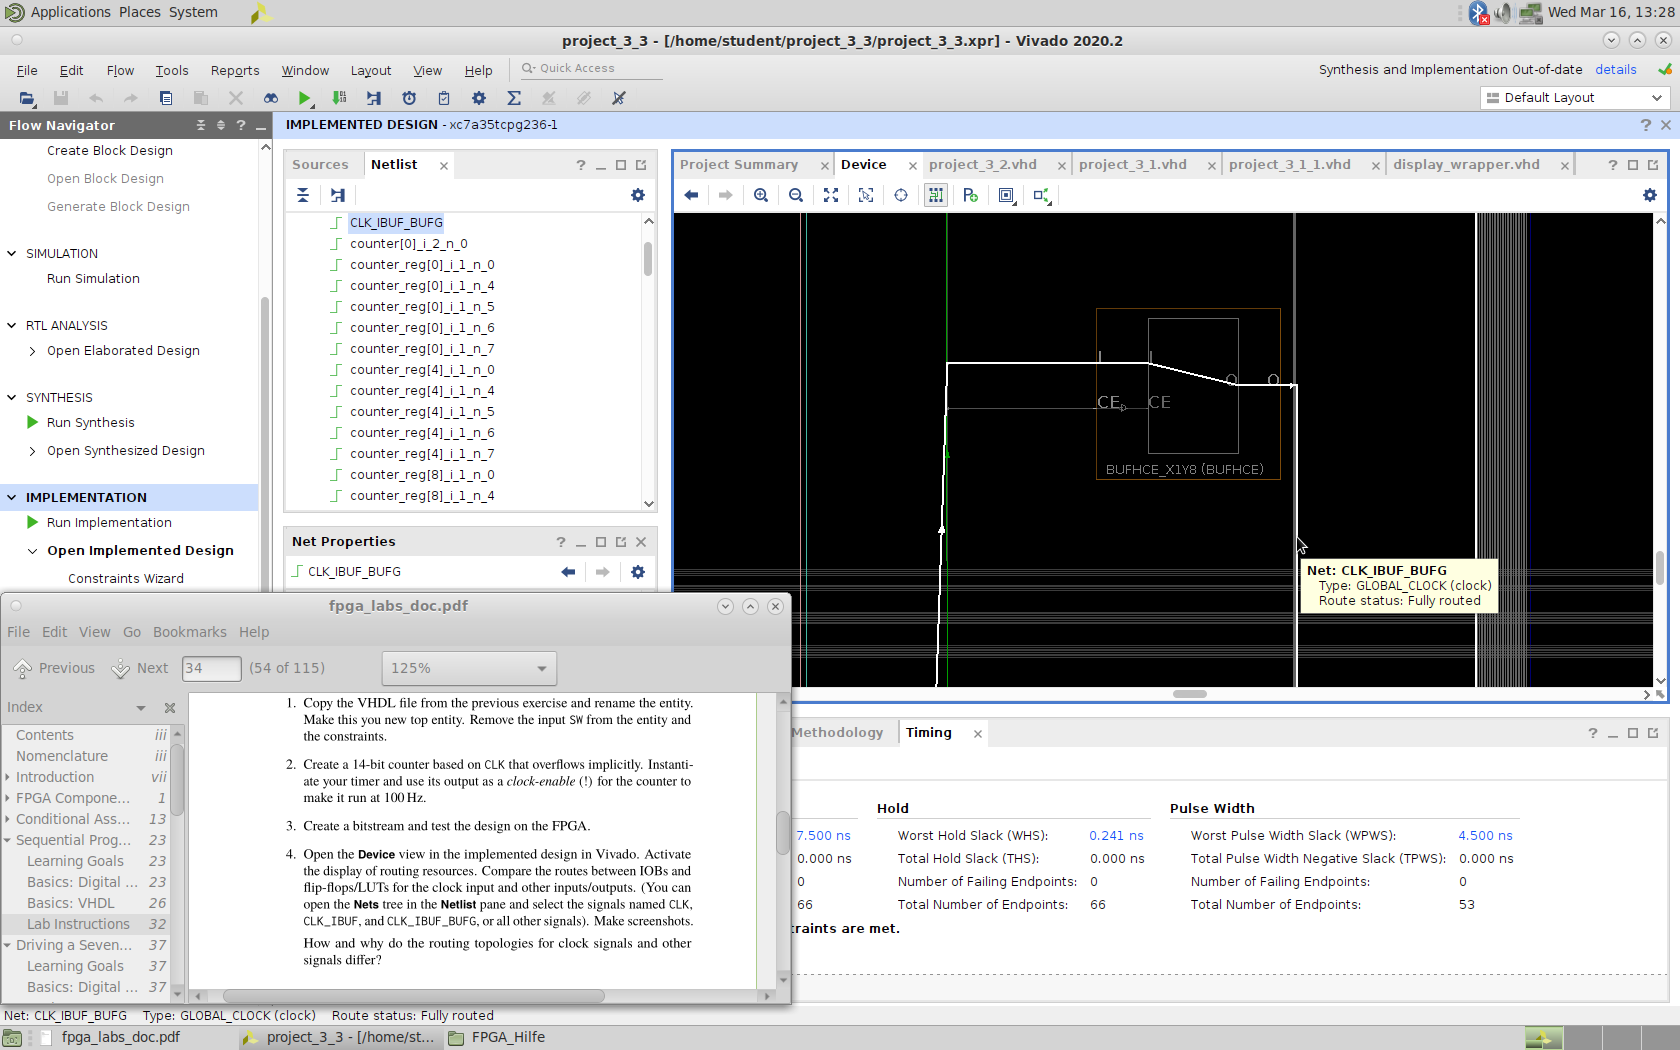
\includegraphics[width=.6\linewidth]{./L3/E3/BUFHCE.png}
	\caption{This clock signal is distributed via these centrally positioned buffer units on the \gls{fpga}.} 
	\label{fig: clock  e_3_3_1}
\end{figure}

\begin{figure}[h]
	\centering
	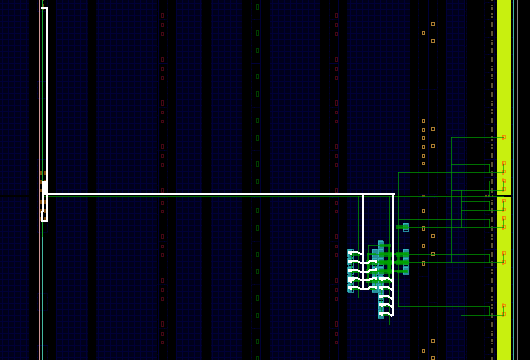
\includegraphics[width=.8\linewidth]{./L3/E3/CLK.png}
	\caption{The distribution of the clock signal. The clock signal is distributed over the central unit on the \gls{fpga} shown in fig. \ref*{fig: clock  e_3_3_1} and in this picture on the top left corner of the image. This design ensures that all the components of the circuit get almost the same clock signal to be in sync.}
	\label{fig: clock routing e_3_3_1}
\end{figure}

%\lstinputlisting[language=VHDL]{./L3/E3/src/project_3_1_1.vhd}

\begin{figure}[h]
	\centering
	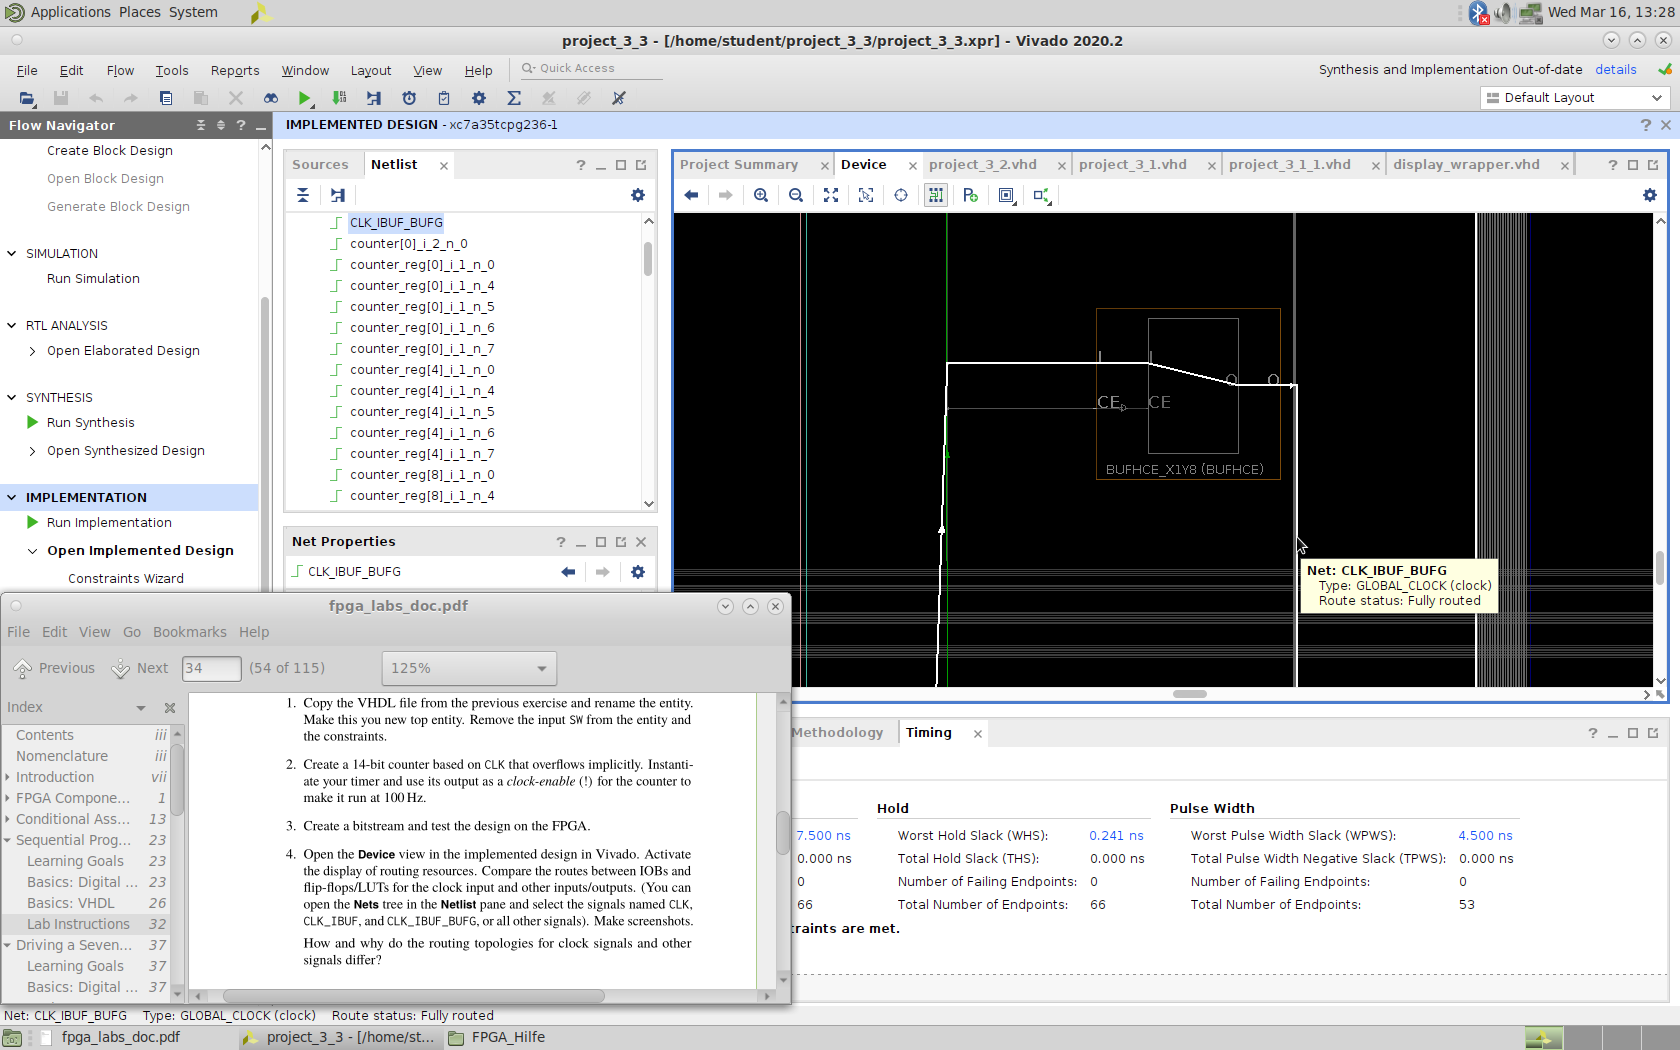
\includegraphics[width=.6\linewidth]{./L3/E3/BUFHCE.png}
	\caption{This clock signal is distributed via these centrally positioned buffer units on the \gls{fpga}.} 
	\label{fig: clock  e_3_3_1}
\end{figure}

\begin{figure}[h]
	\centering
	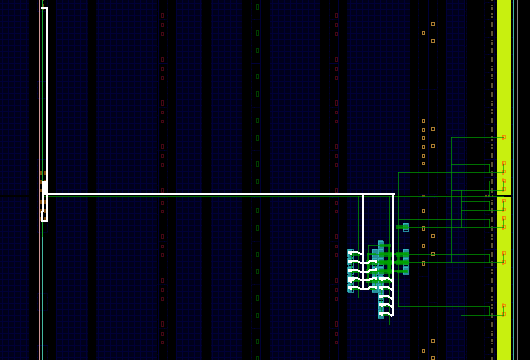
\includegraphics[width=.8\linewidth]{./L3/E3/CLK.png}
	\caption{The distribution of the clock signal. The clock signal is distributed over the central unit on the \gls{fpga} shown in fig. \ref*{fig: clock  e_3_3_1} and in this picture on the top left corner of the image. This design ensures that all the components of the circut get almost the same clock signal to be in sync.}
	\label{fig: clock routing e_3_3_1}
\end{figure}

%\lstinputlisting[language=VHDL]{./L3/E3/src/project_3_1_1.vhd}

%\lstinputlisting[language=VHDL]{./L3/E3/src/project_3_1.vhd}

\lstinputlisting[language=VHDL]{./L3/E3/src/project_3_3.vhd}

The clock signal differs from other signal due to the required equal distribution. Therefore the \gls{fpga} has multiple central distribution units that ensure exactly this as can be seen in fig. \ref{fig: clock routing e_3_3_1}. Otherwise sequential programming cannot work correcly as intended.

The clock signal differs from other signal due to the required equal distribution. Therefore the \gls{fpga} has multiple central distribution units that ensure exactly this as can be seen in fig. \ref{fig: clock routing e_3_3_1}. Otherwise sequential programming cannot work correctly as intended.

\section{Debouncing}

The integrated buttons on the board of the \gls{fpga} have to be debounced in order to be used as an input. As the button bounces up and down multiple times after being pressed only once the ``button-pressed''-status has to be checked with a much lower frequency than the 100\,MHz clock. When pressing the button 20 times and checking the status with the 100\,MHz clock we found that much more than 20 presses were counted. To fix the issue, we found that a 100\,Hz clock fits the job perfectly. Additionally we checked if the button has been pressed in the previous clock cycle of the 100\,Hz clock to eliminate any remaining errors. Checking the program with 50 button presses we found no errors.

\lstinputlisting[language=VHDL]{./L3/E4/src/edge_detector.vhd}


\chapter{Lab 4: Driving a Seven-Segment Display} \label{day4}



\section{Four-byte hex display}

This four-byte hexadecimal display can display a hexadecimal number with up to 4 digits on the display of the \gls{fpga}. In the following module we instantiated the hexadecimal display from lab 2 four times and gave everyone of them four switches of the board. 

Next, we created a timing multiplexer that changes the output and the target digit on the display with 400\,Hz. This frequency enables the display to output a stable image (in this case a number), a lower frequency would lead to flickering. This also means that every digit of the display has a refresh rate of 100\,Hz. Changing the image with the 100\,MHz clock leads to overlapping digits.

\lstinputlisting[language=VHDL]{./L4/E1/src/project_4_1.vhd}

\lstinputlisting[language=VHDL]{./L4/E1/src/project_4_1_1.vhd}

\section{Decimal display for a 14-bit number}

Here, we programmed a binary to decimal converter and used it to input a binary number with the switches of the \gls{fpga} board and output a decimal number on the display. We also use a ``BCD'' converter which converts a binary number into a four bit binary representations of decimal digits. If the number is too large for the display we output an error code. 

The ``BCD'' converter uses the double dabble algorithm from the instructions. For the converter it was beneficial to use the variable data type as it updates continuously after every step during the algorithm rather than being updated once every cycle like a signal.

To output on all four digits on the display, we reuse the previous project. 

\lstinputlisting[language=VHDL]{./L4/E2/src/project_4_2.vhd}

\lstinputlisting[language=VHDL]{./L4/E2/src/BCD.vhd}

\section{Four-byte ASCII display}

Here, we used the same build up as for the hexadecimal display from the first exercise but with an ASCII table. Therefore this module can display various numbers and letters.

\lstinputlisting[language=VHDL]{./L4/E3/src/project_4_3.vhd}

%\lstinputlisting[language=VHDL]{./L4/E3/src/project_2_3_2.vhd}

\section{Multi-purpose display}

The Multi-purpose display has a mode selection input that lets the user chose a given module from the three previous exercises. This enables the display to display all of the above with just one single module. 

The modes are the following :
\begin{itemize}
    \item "00" : 32 bit input that is directly interpreted as 8 bit cathode signals for the four digits.
    \item "01" : The lowest 16 bits are displayed as a four bit hexadecimal number.
    \item "10" : The lowest 14 bits are displayed in their decimal representation.
    \item "11" : The 32 bits are interpreted as 4 ASCII characters.
\end{itemize}

\lstinputlisting[language=VHDL]{./L4/E4/src/project_4_4.vhd}
\chapter{Lab 5: Finite-State Machines} \label{day5}

\section{Three-stage code lock}

In this exercise we programmed a finite state machine using the case statements of ``VHDL''. This three-stage lock uses a code that can be entered to unlock it. The code consists of three numbers and is entered with the switches of the board and every number is confirmed with an enter button. At every point before the third number has been entered the user can return to the first number with an abort button. Every time the code has been entered wrong an error message is shown and if the code has been entered wrong for the third time the lock is closed permanently. And if entered correct after one or two errors the error counter gets reset. If the lock has been opened it can be closed again with the abort button.

Additionally there is a reset button that has been implemented to reset the error counter and to return the lock into its initial unlocked state. And we also implemented a program button that can be used to reprogram the code if the lock is the unlocked state.

\lstinputlisting[language=VHDL]{./L5/src/project_5.vhd}

\chapter{Lab 6: Pulse-Width Modulation} \label{day6}

\section{LED dimmer}

The LED dimmer controls the brightness of an LED by manipulating the duty cycle (DC) of the HIGH signal powering the LED. 

\lstinputlisting[language=VHDL]{./L6/E1/src/project_6_1.vhd}

When the counter reaches the DC limit, the PWM signal goes to 0 and does not power the LED anymore. If the counter reaches the limit, it resets the PWM signal to 1 and the counter to 0 and the process starts again. The brightness of the LED is now dependent on the DC: For a low DC, the LED shines dimm and bright for a DC in the order of the maximum value of the counter. Here we chose a counter with a maximum value of 255.

% DC sollte ein 7 bit Vektor mit 6 downto 0 also einem maximalen Wert von 255 sein.

\lstinputlisting[language=VHDL]{./L6/E1/src/project_6_1_tb.vhd}

This testbench enables us to see the progression of the individual variables, signals as well as in- and outputs. The testbench is a very handy debugging tool of the VIVADO editor. Here the editor simulates the code for a given time and with customizable clocks, in- and outputs. 

\begin{figure}[h]
	\centering
	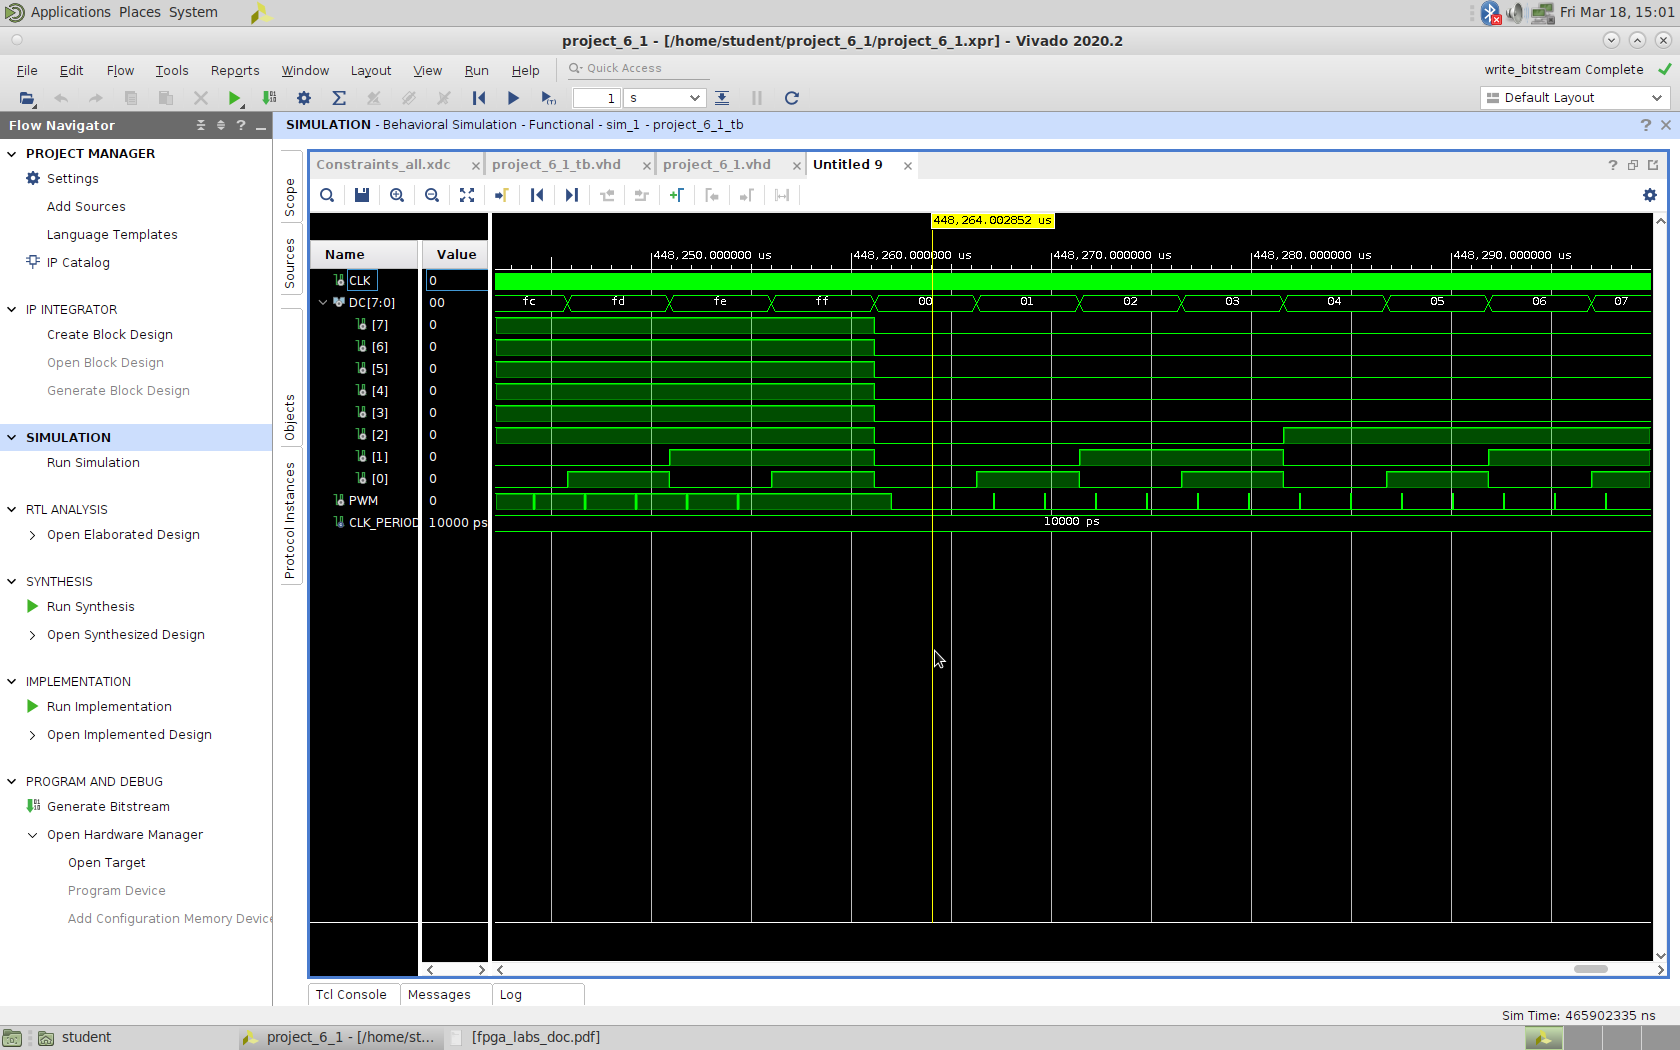
\includegraphics[width=.8\linewidth]{./L6/E1/overflow_time.png}
	\caption{After one full progression the timer is reset to zero.} 
	\label{fig: overflow_time e_6_1 LED dimmer}
\end{figure}

% Wie lange dauert es 1s zu simulieren? Haben wir dazu was aufgeschrieben¿
The simulation takes about 0.5\,s to simulate one second of real time.

\section{Frequency generator}

Next comes a frequency generator. Here, we use the PWM module to generate an audible frequency. Therefore we use a variable frequency and a duty cycle of 50\,\%.

\lstinputlisting[language=VHDL]{./L6/E2/src/project_6_2.vhd}

\lstinputlisting[language=VHDL]{./L6/E2/src/project_6_2_1.vhd}

\lstinputlisting[language=VHDL]{./L6/E2/src/project_6_2_tb.vhd}

After testing the design on the board, we could hear single beats for a frequency of 1\,Hz but we would not consider this a valid sound and the maximum frequency we could hear was between 16000 and 18000\,Hz.

When running the simulation we get a period of 10\,ms for a frequency of 100\,Hz, 1\,ms for 1000\,Hz and 100\,µs for 10000\,Hz. 

\section{Melody}

The following piece of code plays the ``secret'' sound from the ``Legend of Zelda'' games.

\lstinputlisting[language=VHDL]{./L6/E3/src/project_6_3.vhd}

\section{Duty-cycle regulation for a fixed frequency}

Here, we generate a sound with a variable duty cycle and a fixed frequency of 440\,Hz. The variation of the duty cycle enables us to change the speaker volume. The loudest sound can be generated with a duty cycle of 50\,\%. 

% Was haben wir bemerkt als wir die Duty cycle durchgeschaltet haben. Kein linearer Verlauf?

\lstinputlisting[language=VHDL]{./L6/E4/src/project_6_4.vhd}

\lstinputlisting[language=VHDL]{./L6/E4/src/project_6_4_1.vhd}

\section{Duty-cycle regulation for variable frequency}

This program combines the possibility to change the duty cycle and the frequency. Here, we chose to fix the first 6 and last 2 bits of the frequency to 0, so in total the frequency has a range from 128 to 16383\,Hz and 0\,Hz. The duty cycle can be regulated form 0 to 100\,\% with a step size of 1/255 $\approx$ 0.2\,\%.

% auch hier möglicherweise auf 255 ändern

\lstinputlisting[language=VHDL]{./L6/E5/src/project_6_5.vhd}

\lstinputlisting[language=VHDL]{./L6/E5/src/project_6_5_1.vhd}

\chapter{Lab 7: UART} \label{day7}

\section{Direct loop-back}

\lstinputlisting[language=VHDL]{./L7/E1/src/project_7_1.vhd}

\section{UART sender}

\lstinputlisting[language=VHDL]{./L7/E2/src/project_7_2.vhd}

\lstinputlisting[language=VHDL]{./L7/E2/src/project_7_2_1.vhd}

\section{Simple UART receiver}

\lstinputlisting[language=VHDL]{./L7/E3/src/project_7_3.vhd}

\lstinputlisting[language=VHDL]{./L7/E3/src/project_7_3_1.vhd}

\lstinputlisting[language=VHDL]{./L7/E3/src/project_7_3_tb.vhd}

\section{Oversampling UART receiver}

\lstinputlisting[language=VHDL]{./L7/E3/src/project_7_3.vhd}

\lstinputlisting[language=VHDL]{./L7/E3/src/project_7_3_1.vhd}

\chapter{Lab 8: Memory} \label{day8}

\section{Memory module}

This module can store and output stored information. The data to be stored is received using the ``UART''-receiver module from the previous lab and then read out from the memory and displayed on the display of the \gls{fpga} board after pressing a button. 

The module can store 256 bytes. After 256 bytes the write address overflows and starts to overwrite information. The read address can be selected with switches and displayed after pressing a button.

\lstinputlisting[language=VHDL]{./L8/E1/src/project_8_1.vhd}

\lstinputlisting[language=VHDL]{./L8/E1/src/project_8_1_1.vhd}

\section{LIFO/stack}

The ``LIFO'' stack works as follows: The last stored information ist the first to be output. We use it here to display the received information from the computer keyboard on the display of the \gls{fpga} after pressing the button.

\lstinputlisting[language=VHDL]{./L8/E2/src/project_8_2.vhd}

\lstinputlisting[language=VHDL]{./L8/E2/src/project_8_2_1.vhd}

Additionally we test several borderline cases: 

\begin{itemize}
    \item reading from an empty stack
    \item writing to a full stack
    \item simultaneous reading and writing (starting with a full/empty stack)
\end{itemize}

\begin{figure}
    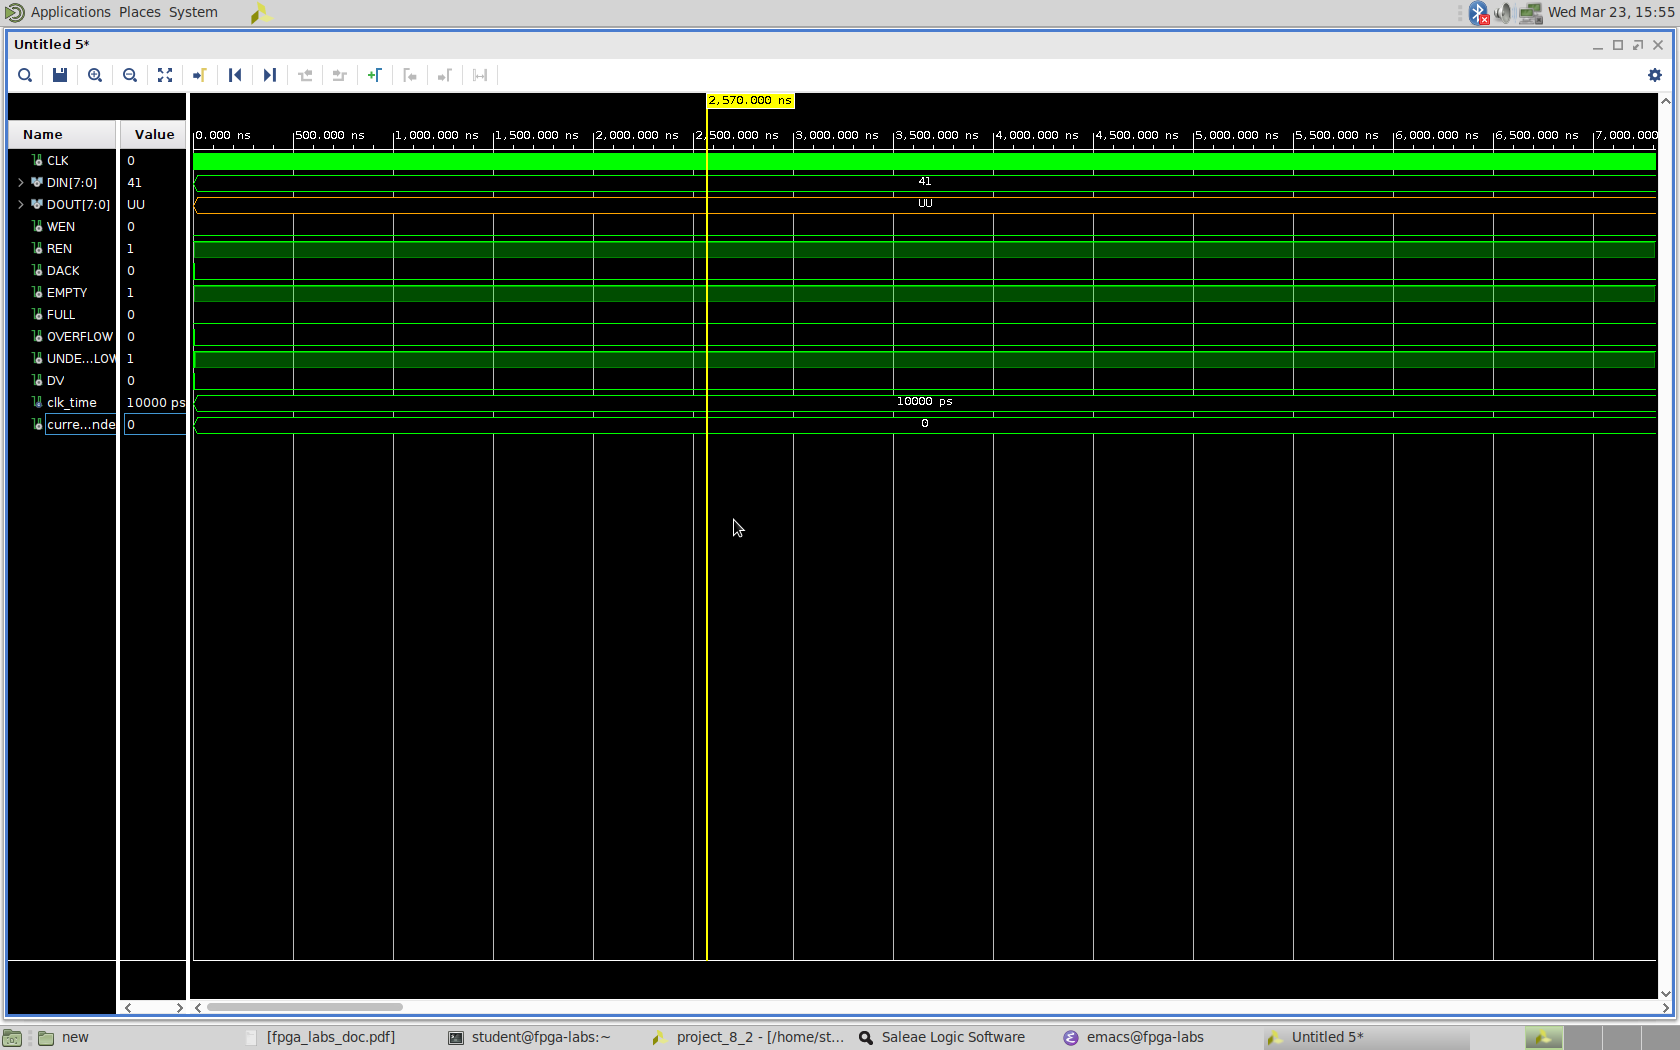
\includegraphics[width=.9\textwidth]{L8/E2/underflow.png}
    \caption{Reading from an empty stack. The stack underflows.}
    \label{pic: reading from an empty stack}
\end{figure}

\begin{figure}
    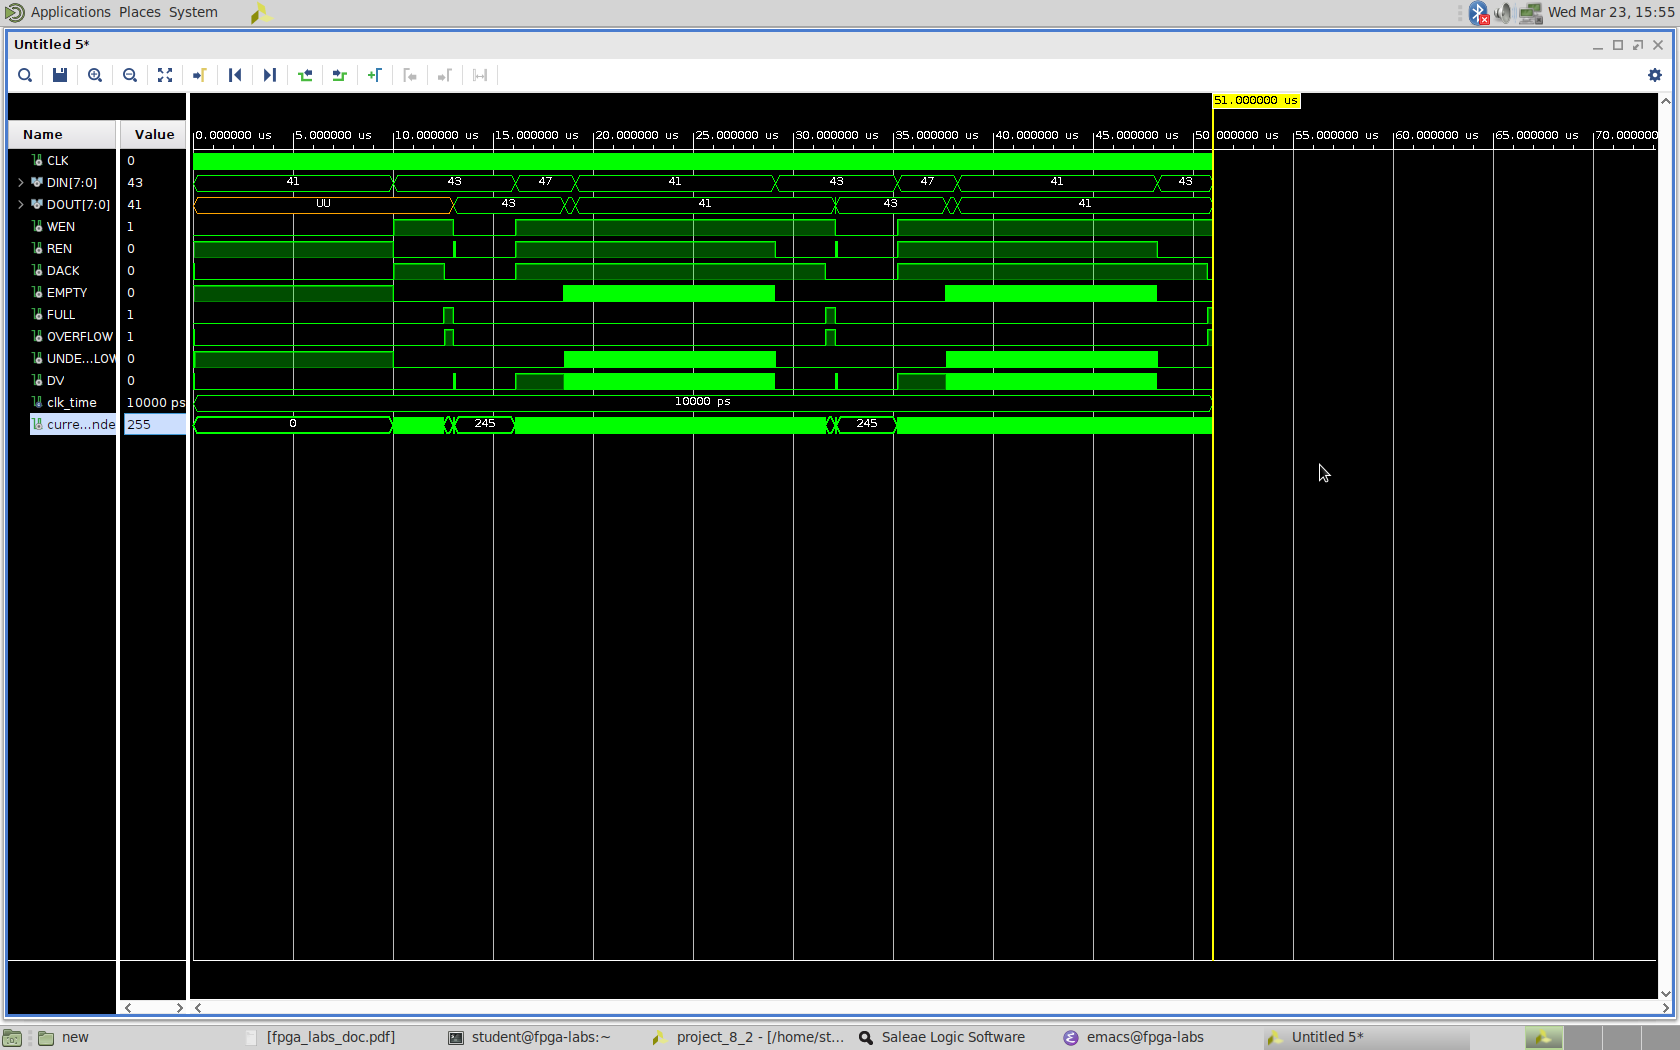
\includegraphics[width=.9\textwidth]{L8/E2/full.png}
    \caption{Writing to a full stack. The stack overflows and information is overwritten.}
    \label{pic: writing to a full stack}
\end{figure}

\begin{figure}
    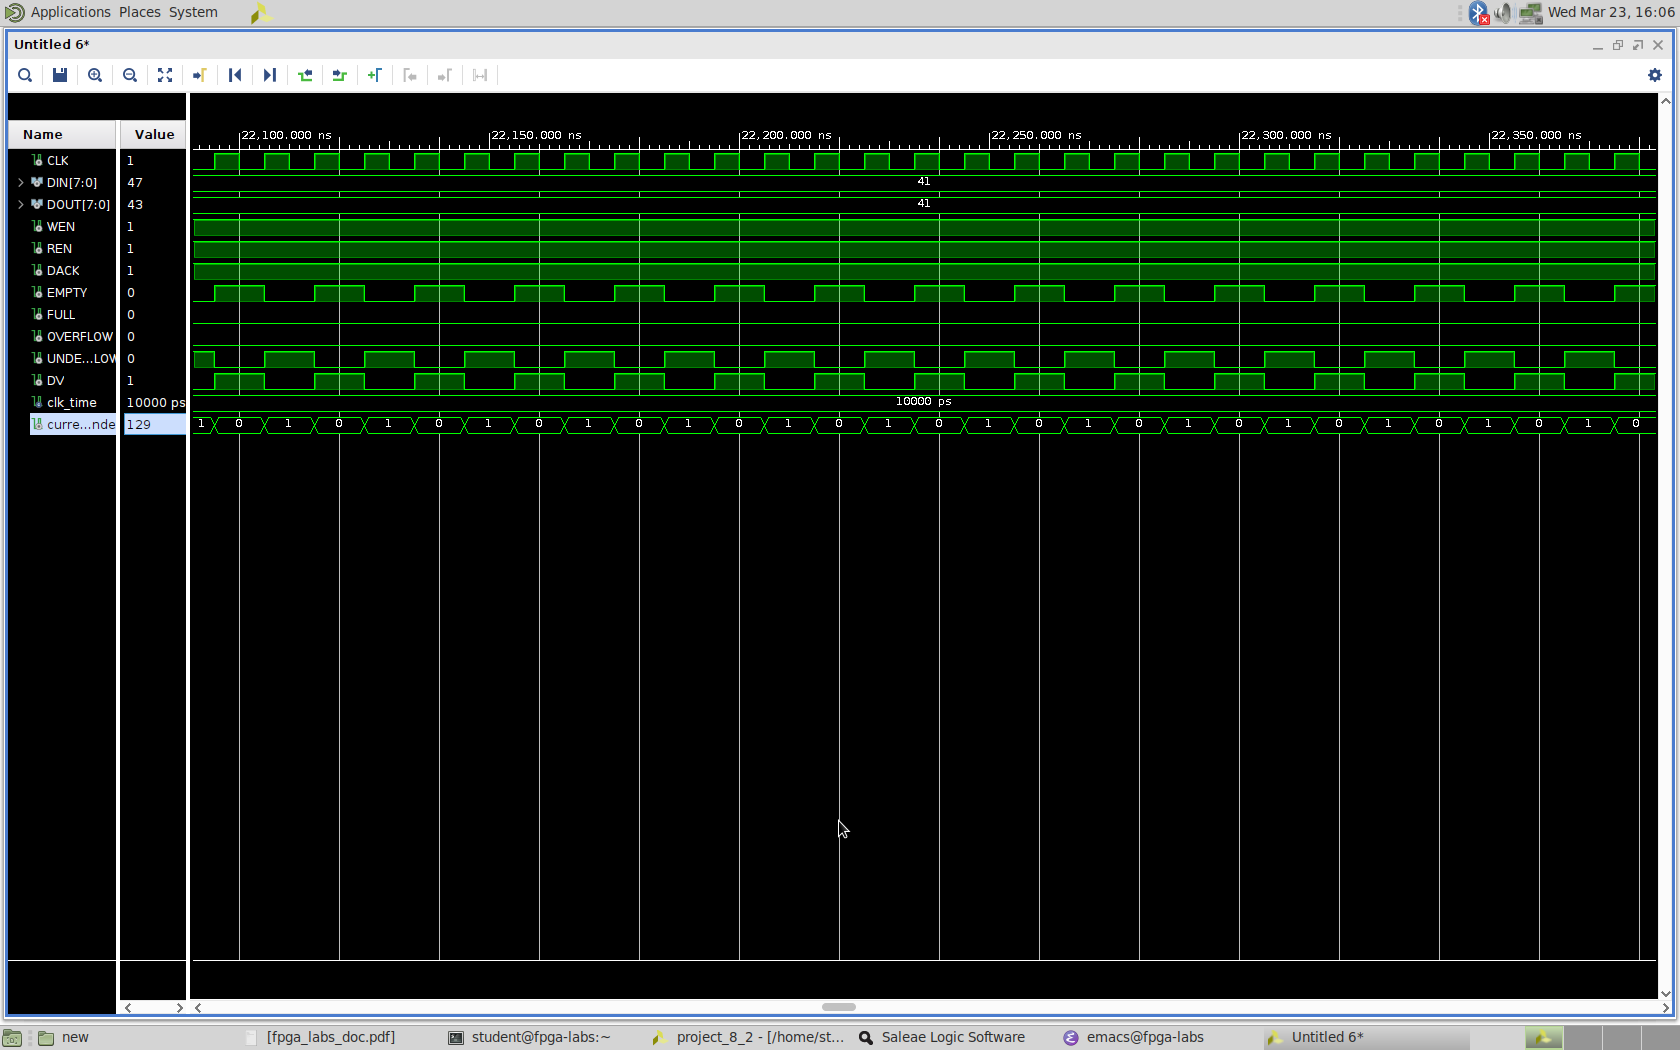
\includegraphics[width=.9\textwidth]{L8/E2/sim_read_write_underflow_empty.png}
    \caption{Writing and reading from an empty stack. The current address number oscillates between 0 and 1.}
    \label{pic: w and r from e stack}
\end{figure}

\begin{figure}
    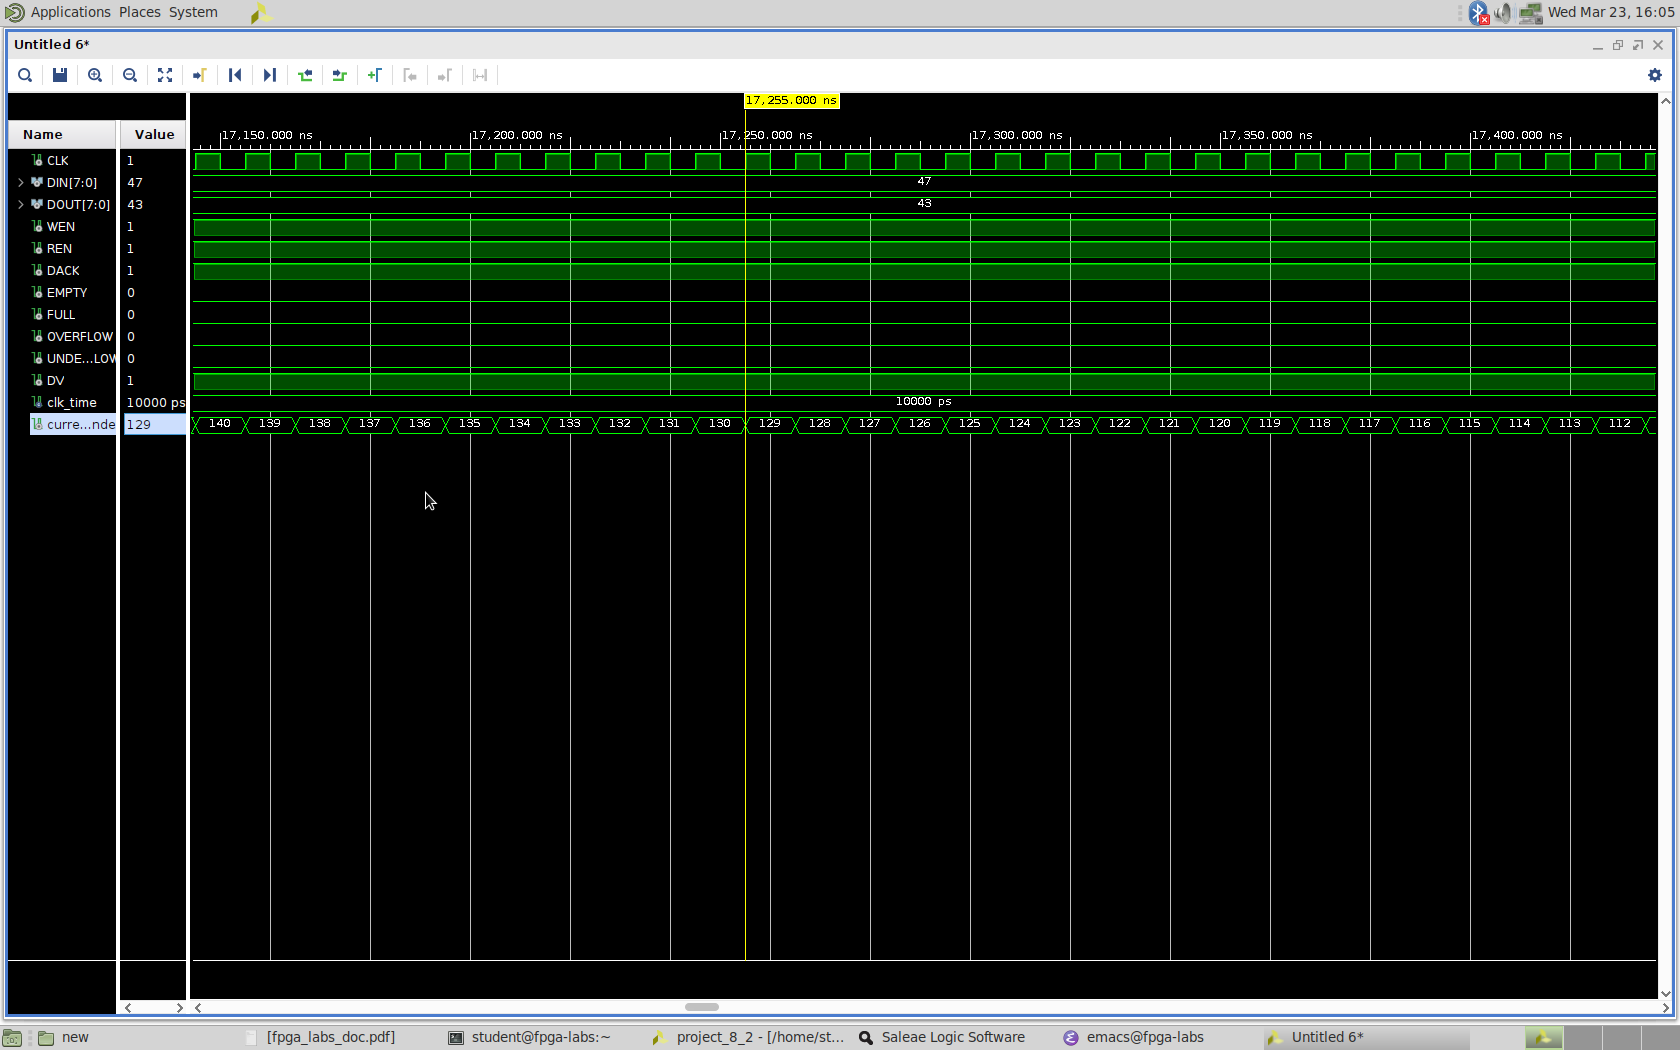
\includegraphics[width=.9\textwidth]{L8/E2/sim_read_write_full.png}
    \caption{Writing and reading from a full stack. The current address number goes down.}
    \label{pic: w and r from f stack}
\end{figure}

\newpage

\section{FIFO/queue}

The FIFO or queue module outputs the information in the exact order initially input to the memory. This is done with two pointers. One pointer for the input and one for the output.

\lstinputlisting[language=VHDL]{L8/E3/src/project_8_3.vhd}

%\lstinputlisting[language=VHDL]{L8/E3/src/project_8_2_1.vhd}

%\lstinputlisting[language=VHDL]{L8/E3/src/project_8_2_tb.vhd}

Again we simulated the borderline cases:

\begin{figure}
    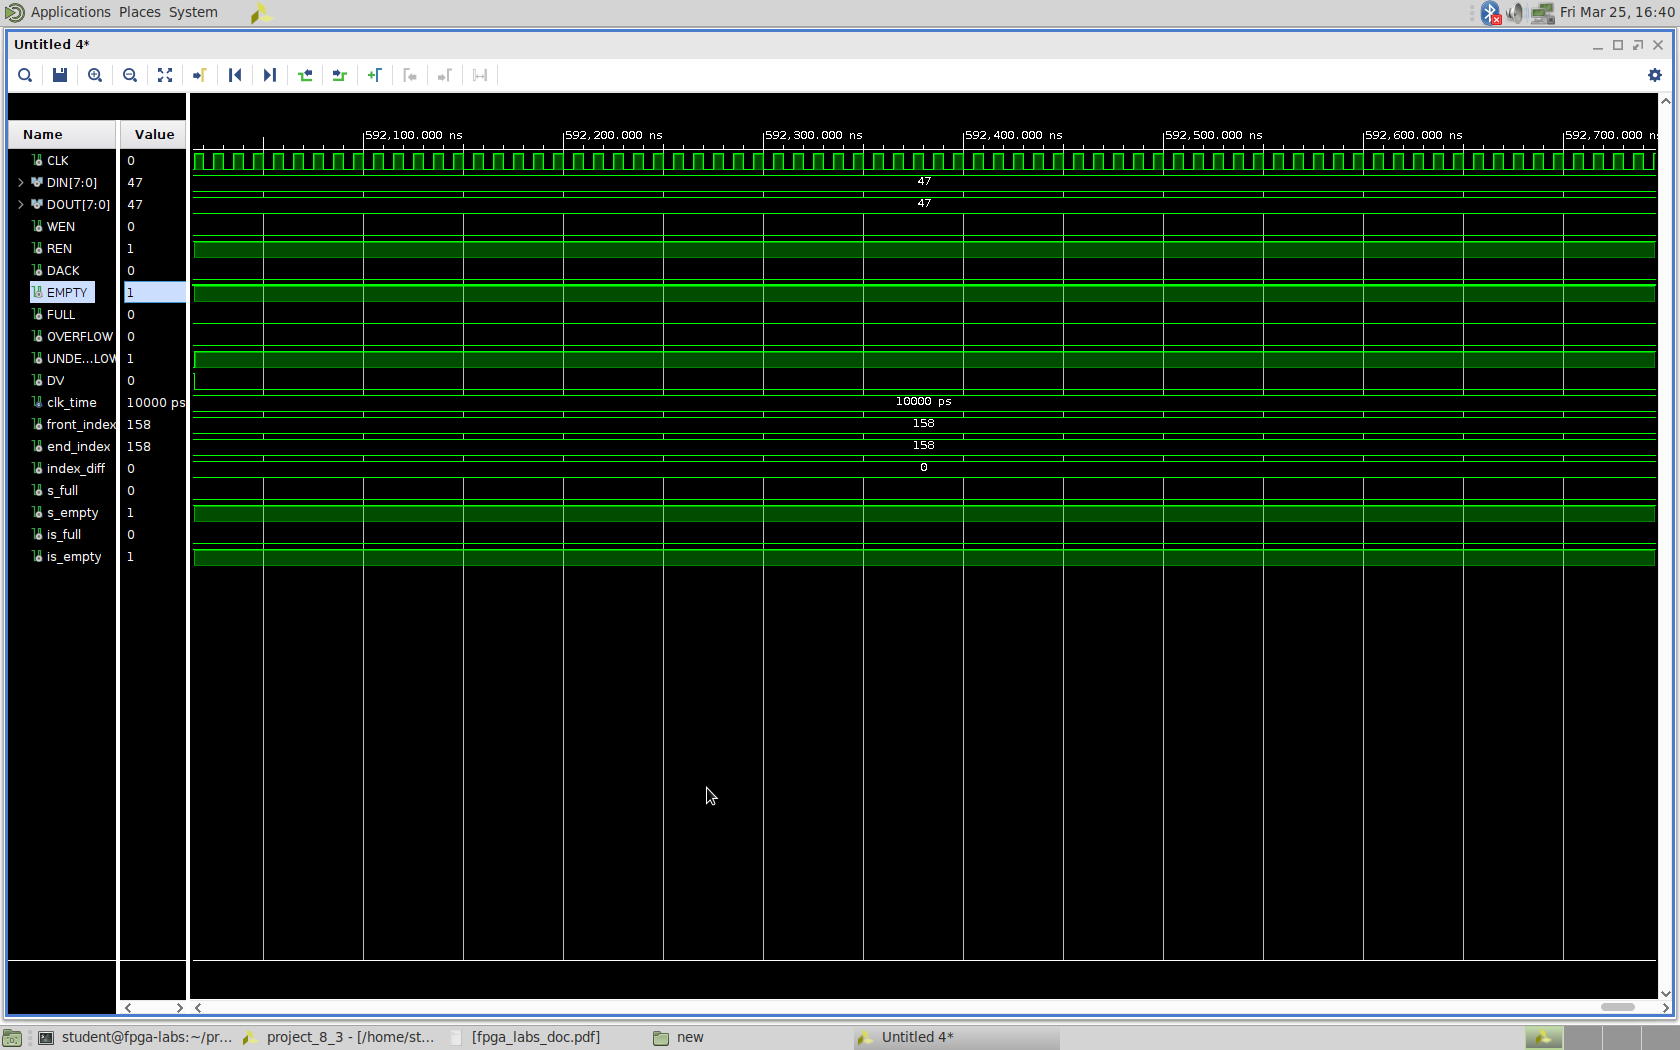
\includegraphics[width=.9\textwidth]{L8/E3/empty_read.png}
    \caption{Reading from an empty stack. The module returns that it is empty and underflows.}
    \label{pic: r from e stack fifo}
\end{figure}

\begin{figure}
    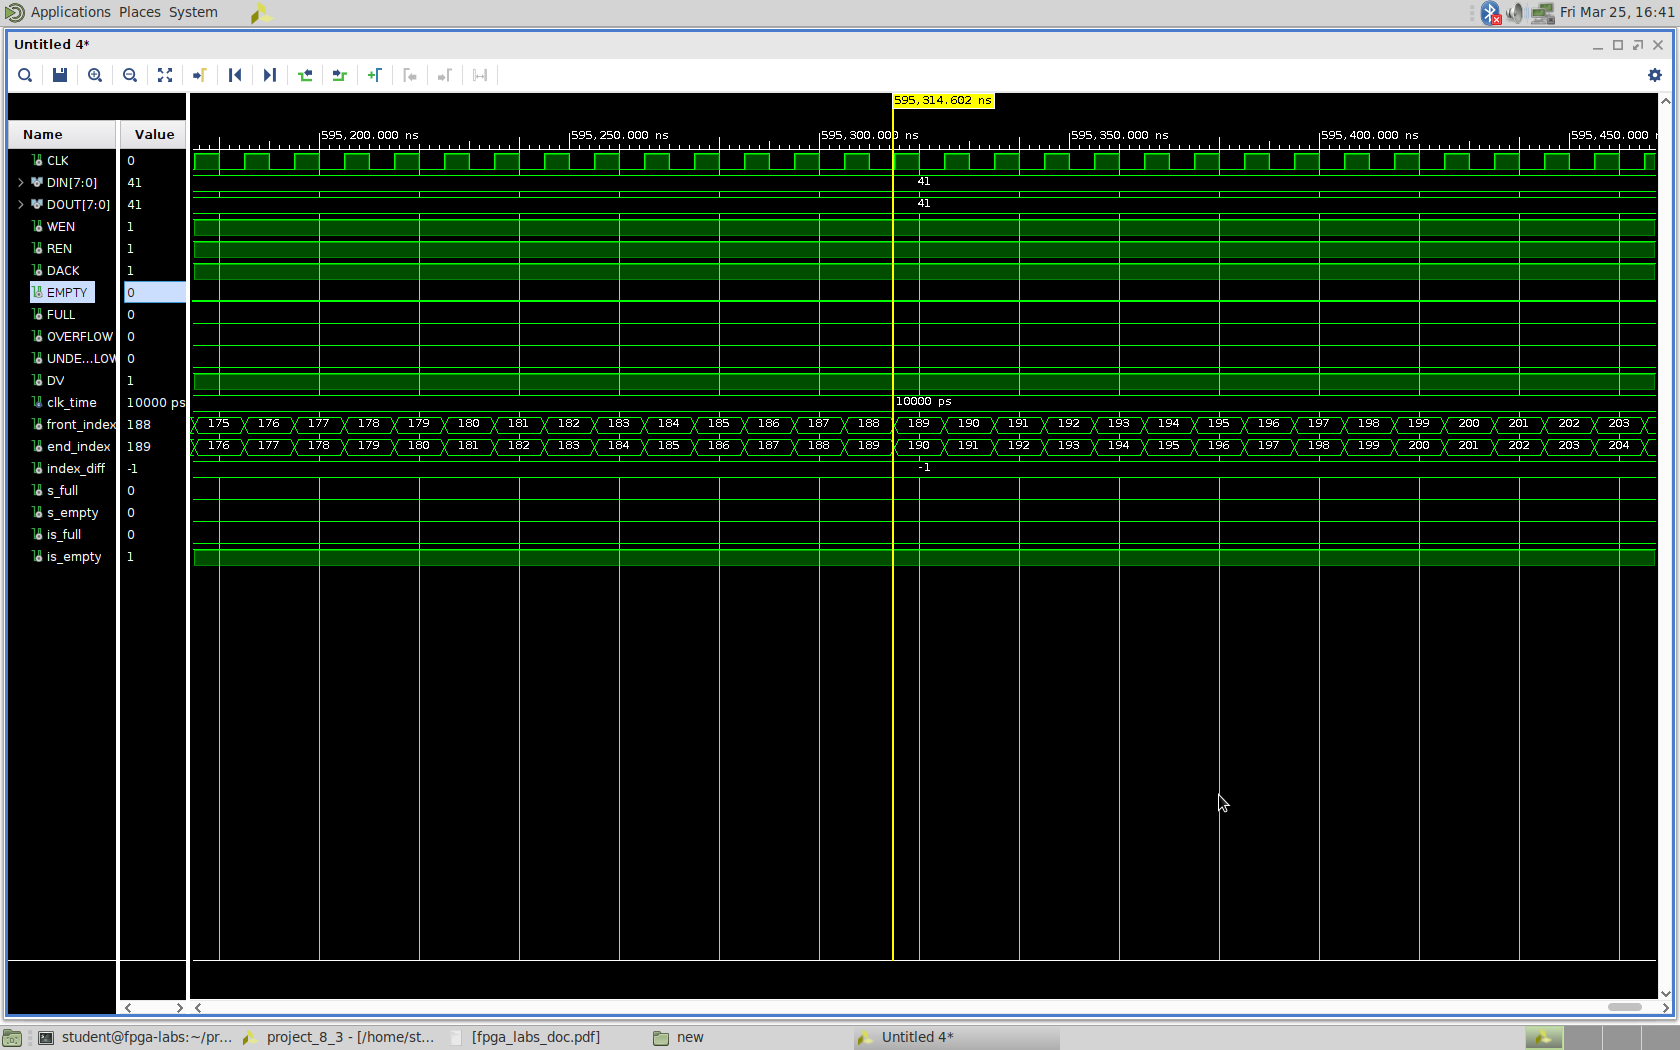
\includegraphics[width=.9\textwidth]{L8/E3/read_and_write_sametime.png}
    \caption{Simultaneous reading an writing. The module writes and reads correctly at the same time.}
    \label{pic: r and e from half stack fifo}
\end{figure}

\begin{figure}
    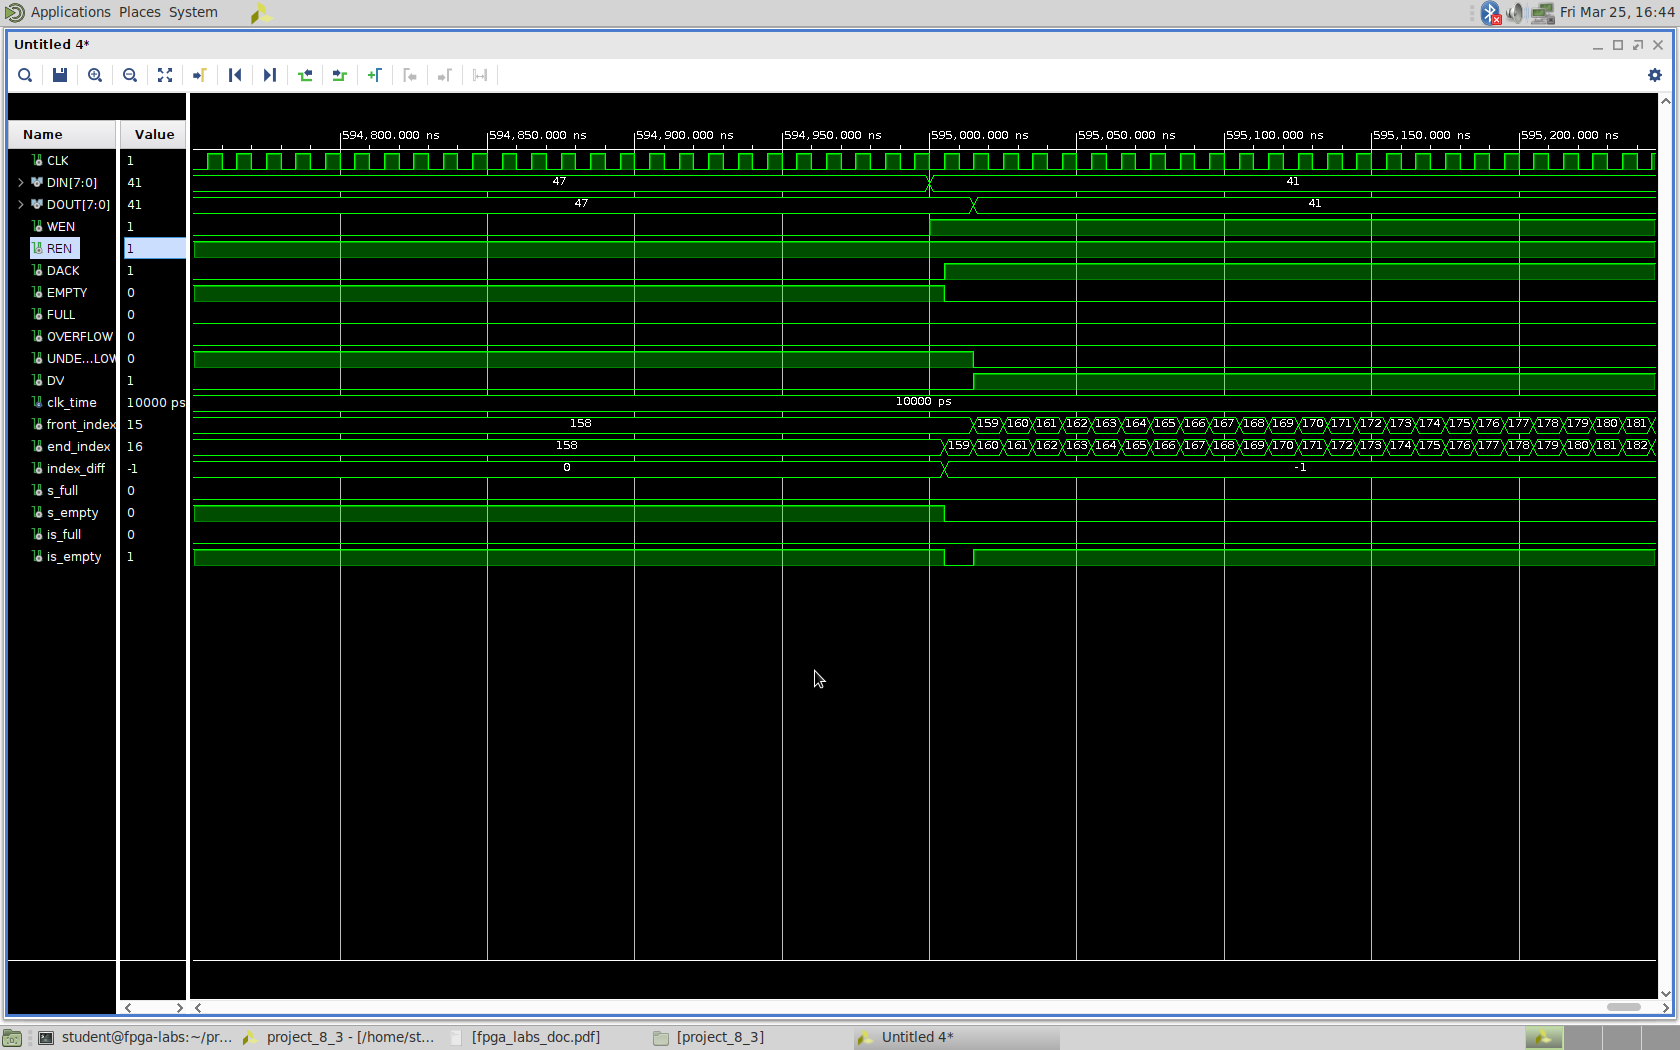
\includegraphics[width=.9\textwidth]{L8/E3/read_write_from_empty.png}
    \caption{Simultaneous reading an writing from empty stack. The end index (which is used as the write index) moves one up and the front index stays the same. It then shows the same behavior as before.}
    \label{pic: r and e from e stack fifo}
\end{figure}

\begin{figure}
    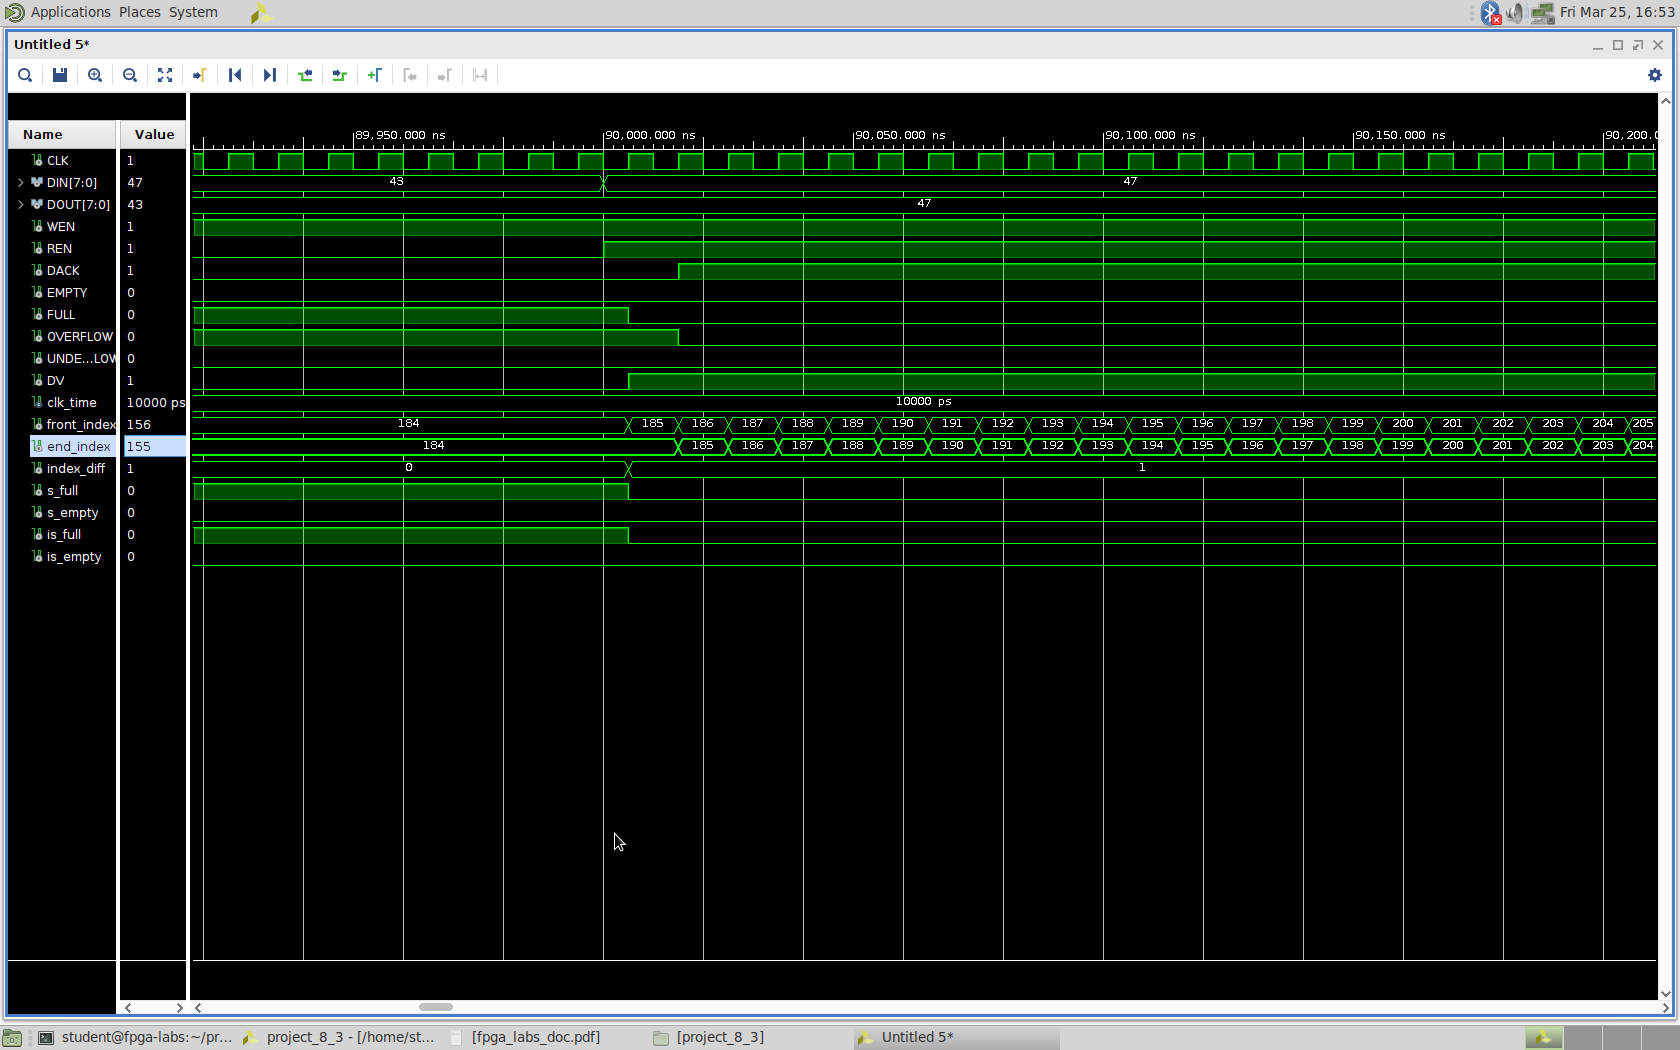
\includegraphics[width=.9\textwidth]{L8/E3/read_write_from_full.png}
    \caption{Simultaneous reading an writing from full stack. Here, the read index moves first and as free space is available again the write index moves upwards.}
    \label{pic: r and e from f stack fifo}
\end{figure}

\begin{figure}
    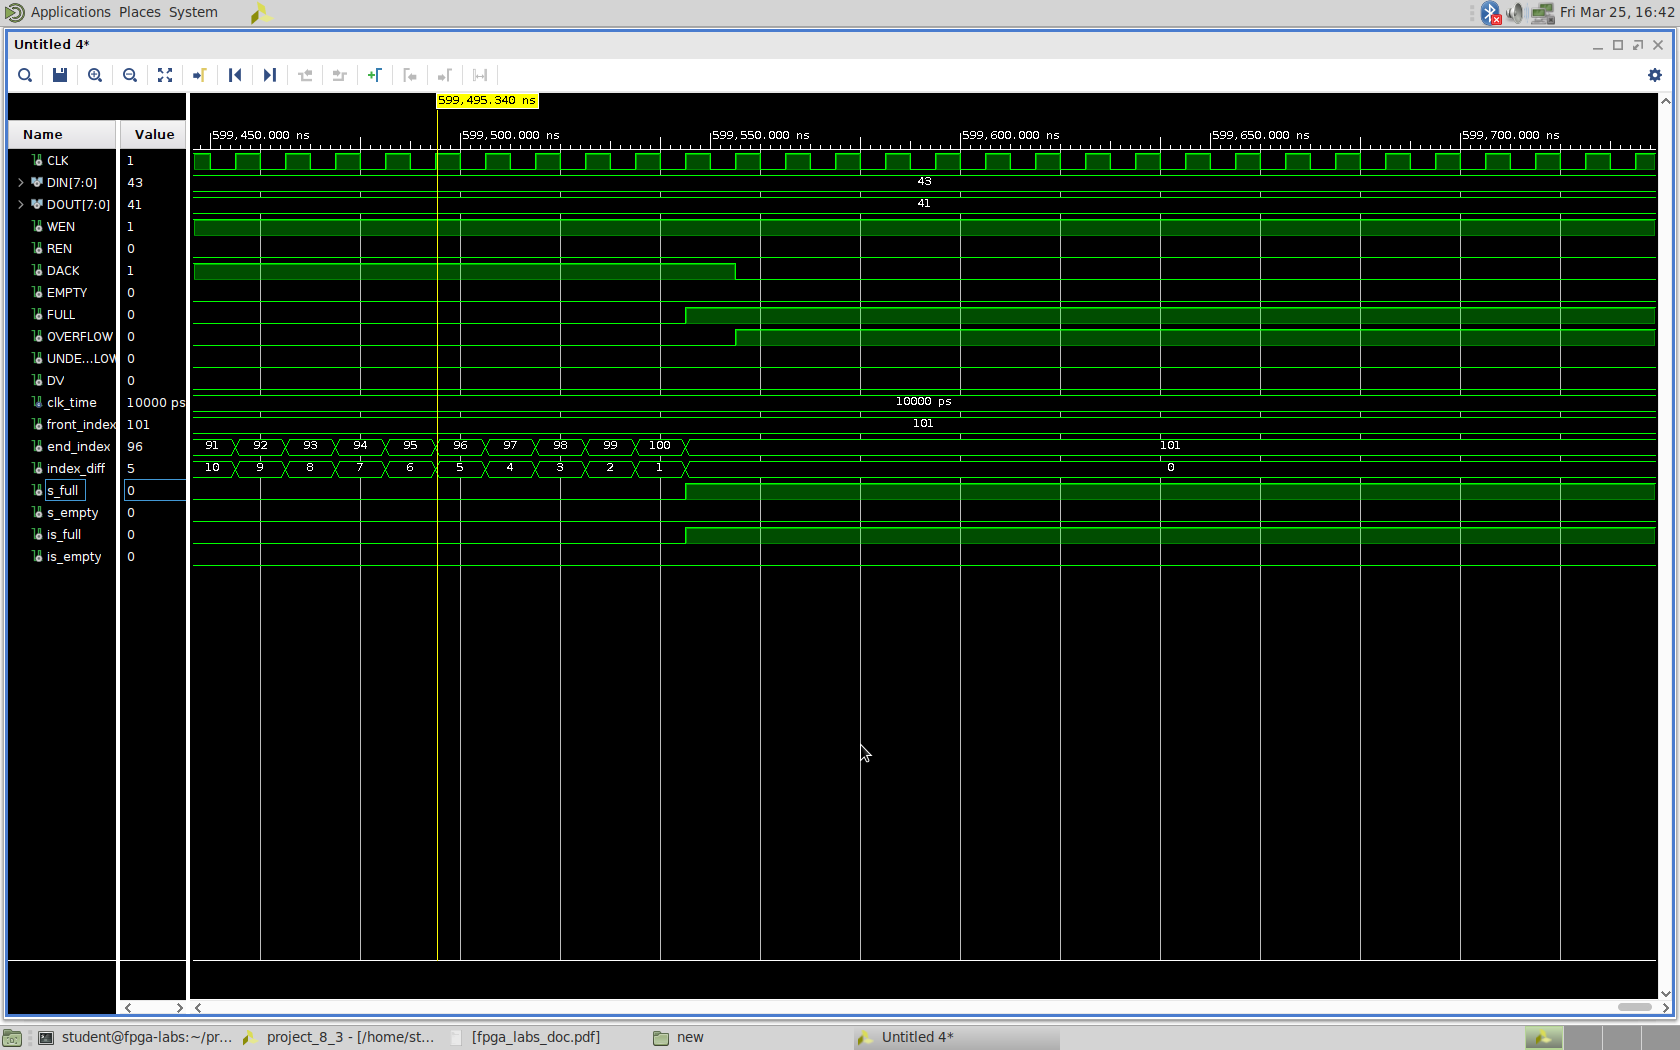
\includegraphics[width=.9\textwidth]{L8/E3/write_overflow.png}
    \caption{Writing to a full stack. The stack overflows.}
    \label{pic: r to f stack fifo}
\end{figure}
\chapter{Lab 9: Driving a VGA Monitor}

\section{Solid color}

This module is our main setup for the display. It includes all timings necessary to display a solid color on our display with HD+ resolution.

\lstinputlisting[language=VHDL]{./L9/E1/src/project_9_1.vhd}

\section{Patterns}

Here, we created two animated and three static patterns: an animated circle and a shifting colors pattern as well as a checkerboard, circles and stripes.

\lstinputlisting[language=VHDL]{./L9/E2/src/animated_circle.vhd}

\lstinputlisting[language=VHDL]{./L9/E2/src/shifting_colors.vhd}

\lstinputlisting[language=VHDL]{L9/E2/src/checkboard.vhd}

\lstinputlisting[language=VHDL]{L9/E2/src/circles.vhd}

\lstinputlisting[language=VHDL]{L9/E2/src/stripes.vhd}

\section{Video memory}

This module comes with a preloaded image that is saved to the ram of the \gls{fpga} and then displayed on a screen. Therefore we used the init$\_$ram function of VHDL from the instructions. Before that, the image has been converted to a black and white image to meet the RAM limitations (max. 1.800\,Kb) of the \gls{fpga}.

\lstinputlisting[language=VHDL]{L9/E3/src/project_9_3.vhd}

\lstinputlisting[language=VHDL]{L9/E3/src/video_memory.vhd}

\section{Video data from UART}

Here, we used UART to transmit data to the video memory of the \gls{fpga}. After converting a picture to a black and white image it can be transmitted with the terminal tool.

\lstinputlisting[language=VHDL]{L9/E4/src/project_9_4.vhd}

\backmatter
% bibliography, glossary and index would go here.

\end{document}